\clearpage
\section{Konzept}\label{sec:Konzept}

Für den Vergleich der 3 Mesh Netzwerkstacks Bluetooth Mesh (BT Mesh), Thread und Zigbee wird ein vom Mesh Protokoll unabhängiges Testkonzept umgesetzt welches in der Abbildung \ref{fig:MeshTestKonzept} als Konzeptschema dargestellt ist. Die Benchmark Slave Nodes (BSN) in der Abbildung als Sensoren und Aktoren mit unterschiedlichen Funktionalitäten dargestellt, bilden zusammen mit dem Benchmark Master Node (BMN) das zu testende Mesh Netzwerk. Innerhalb des Netzwerks wird dessen Organisation vom jeweiligen Protokoll sichergestellt. Das Testnetzwerk soll ein realitätsnahes Netzwerk nachbilden. Beispielsweise wird eine Hausautomation in einem Einfamilienhaus als Referenz angenommen in welchem jeweils nur gewisse Nodes untereinander Applikationsdaten austauschen. Ein Lichtschalter kommuniziert nur mit einer Lichtquelle und umgekehrt. Der selbe Lichtschalter tauscht jedoch keine Applikationsdaten mit dem Temperatursensor aus. Trotzdem bilden die Nodes zusammen ein Mesh Netzwerk. Diese unterschiedlichen Beziehungen innerhalb des Mesh Netzwerks sind in der Abbildung \ref{fig:MeshTestKonzept} bereits angedeutet und werden im Abschnitt \ref{subsec:MeshBeziehungen} noch genauer beschrieben.

Die Benchmark Management Station (BMS) welche mit dem BMN via USB/UART kommuniziert, ist zuständig für die Verwaltung und Verarbeitung der Benchmarks. Während eines Benchmark Prozesses sollen sämtliche Messungen jedoch unabhängig von der BMS durchgeführt werden damit allfällige Latenzzeiten der USB/UART Verbindung die Resultate nicht verfälschen.



\begin{figure}[H]
	\centering
	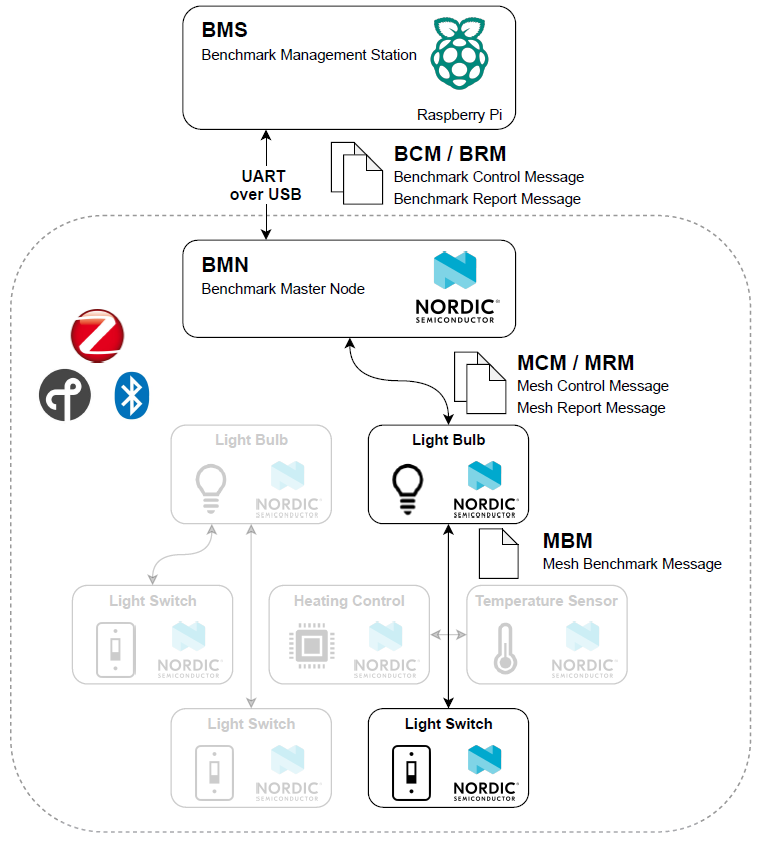
\includegraphics[width=0.7\textwidth]{Mesh_Testkonzept.png}
	\caption{Konzeptschema für den Ablauf eines Mesh Benchmarks.}\label{fig:MeshTestKonzept}
\end{figure}


In der Abbildung \ref{fig:MeshTestKonzept} sind verschiedene Messages dargestellt. Dabei handelt es sich um die Nachrichten die zwischen den einzelnen Teilen des Testaufbaus versendet werden und schliesslich einen Benchmark ausmachen. Die Messages besitzen Funktionen:

\paragraph{Mesh Benchmark Message (MBM)}
Die MBM ist jene Message welche die eigentlichen Messdaten produziert und diese sogleich unter den BSN (Mesh Knoten) überträgt. Anhand dieser Messages werden die Parameter gemäss der Messwerttabelle in Anhang \ref{app:MesswerteBenchmarkMeshNetzwerke} erfasst. Bei den MBM handelt es sich also eigentlich um eine Sammlung von Messages welche je nach gewünschtem Messwert in Form und Anzahl unterschiedlich ausfallen können.



\paragraph{Mesh Control Message (MCM)}
Die MCM beinhaltet die Parameter für die Benchmarks welche vom BMN an die BSN übertragen werden. Ausserdem werden damit Kontrollbefehle für die Benchmarks wie beispielsweise \textit{Start/Stop} sowie \textit{Laufzeit, Wiederholrate usw.} übertragen.




\paragraph{Mesh Report Message (MRM)}



\paragraph{Benchmark Control Message (BCM)}



\paragraph{Benchmark Report Message (BRM)}




